\section{Goals and Contribution}

The goal of this thesis is divided into two parts. The first part is to develop an Android application for the paper, "Publish/Subscribe for Mobile Applications using Shared Dictionary Compression" \parencite{sdcdemo}. The application will provide the provision to subscribe to a set of topics. Each topic would correspond to messages being received by the Android application in different formats such as JSON, XML, and CSV. The messages would contain location coordinates which will be displayed on a map. The Android application would also demonstrate the throughput comparison with and without the use of SSPS.

The next part of the thesis is to solve the problem of the Sampling Broker being a centralized entity. In general, the problem of a centralized system is solved by replacing it with a distributed system \parencite{tanenbaum2007distributed}. Hence, in this case, the idea is to replace the centralized broker with a distributed broker. Currently, there exists no implementation of SSPS on any of the available distributed brokers.

There are several open-source distributed brokers like Apache ActiveMQ Artemis, Apache Kafka and so on. The first step will be to study the different open-source distributed brokers and select one of them for implementing the SSPS. In the second step, once an appropriate broker has been chosen, the architecture of the broker needs to be understood in order to extend it to incorporate the SSPS. Finally, the last step will involve design and implementation of a prototypical extension for the distributed broker to incorporate SSPS. Figure \ref{figures:dist_ssps} depicts the design of the SSPS model in the case of a distributed broker. In comparison to Figure \ref{figures:ssps} it can be seen that now there are several instances of the sampling broker instead of only one instance.

\makeatletter
\setlength{\@fptop}{0pt}
\makeatother

\begin{figure}[t!]
\centering
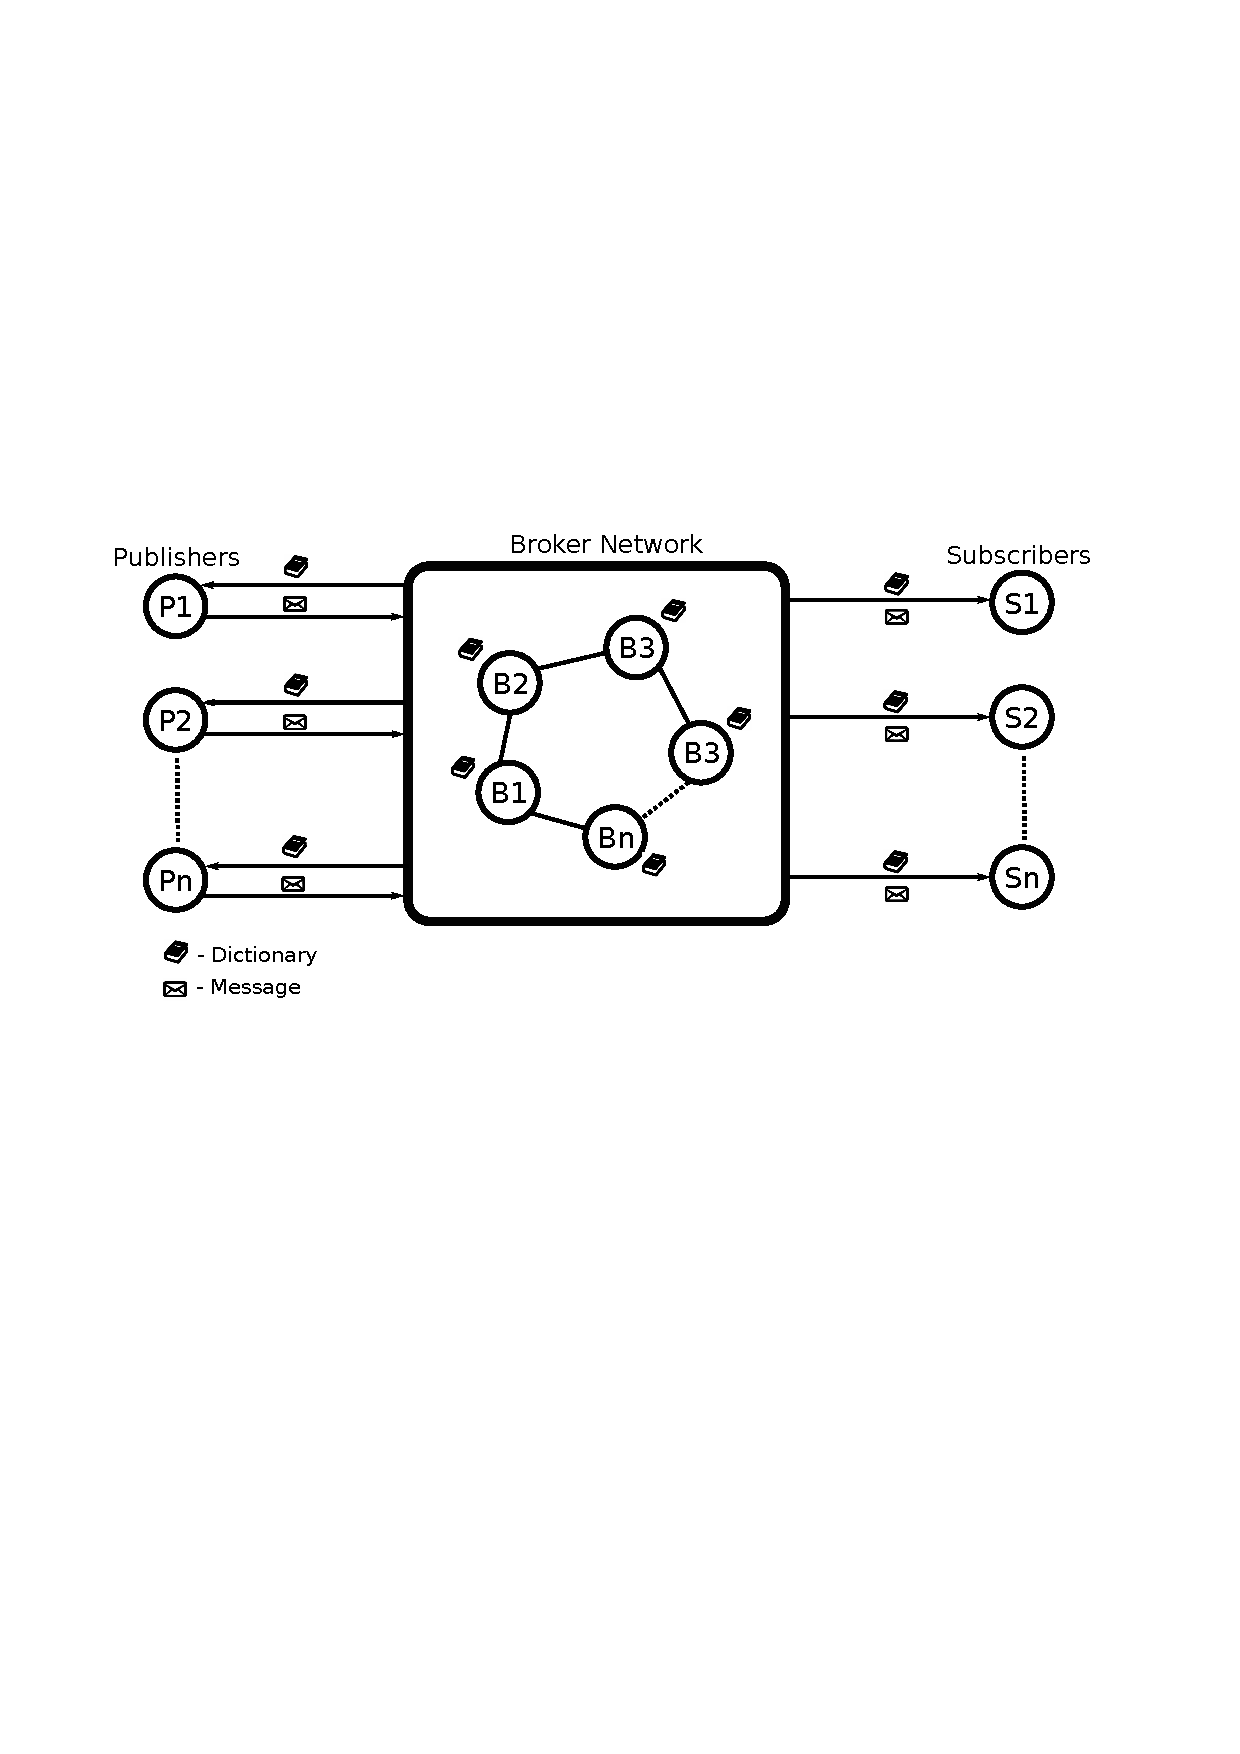
\includegraphics[keepaspectratio, width=.9\textwidth, trim={0 12cm 0 9cm},clip]{dist_ssps.pdf}
\caption{SSPS in a distributed broker}\label{figures:dist_ssps}
\end{figure}

On completion of implementation, the prototypical implementation will be tested to get performance aspects such as throughput, CPU and memory usage and behavioral aspects such as the effect of SSPS in the case of failover.
